% Options for packages loaded elsewhere
\PassOptionsToPackage{unicode}{hyperref}
\PassOptionsToPackage{hyphens}{url}
\PassOptionsToPackage{dvipsnames,svgnames,x11names}{xcolor}
%
\documentclass[
  letterpaper,
  DIV=11,
  numbers=noendperiod]{scrreprt}

\usepackage{amsmath,amssymb}
\usepackage{lmodern}
\usepackage{iftex}
\ifPDFTeX
  \usepackage[T1]{fontenc}
  \usepackage[utf8]{inputenc}
  \usepackage{textcomp} % provide euro and other symbols
\else % if luatex or xetex
  \usepackage{unicode-math}
  \defaultfontfeatures{Scale=MatchLowercase}
  \defaultfontfeatures[\rmfamily]{Ligatures=TeX,Scale=1}
\fi
% Use upquote if available, for straight quotes in verbatim environments
\IfFileExists{upquote.sty}{\usepackage{upquote}}{}
\IfFileExists{microtype.sty}{% use microtype if available
  \usepackage[]{microtype}
  \UseMicrotypeSet[protrusion]{basicmath} % disable protrusion for tt fonts
}{}
\makeatletter
\@ifundefined{KOMAClassName}{% if non-KOMA class
  \IfFileExists{parskip.sty}{%
    \usepackage{parskip}
  }{% else
    \setlength{\parindent}{0pt}
    \setlength{\parskip}{6pt plus 2pt minus 1pt}}
}{% if KOMA class
  \KOMAoptions{parskip=half}}
\makeatother
\usepackage{xcolor}
\setlength{\emergencystretch}{3em} % prevent overfull lines
\setcounter{secnumdepth}{5}
% Make \paragraph and \subparagraph free-standing
\ifx\paragraph\undefined\else
  \let\oldparagraph\paragraph
  \renewcommand{\paragraph}[1]{\oldparagraph{#1}\mbox{}}
\fi
\ifx\subparagraph\undefined\else
  \let\oldsubparagraph\subparagraph
  \renewcommand{\subparagraph}[1]{\oldsubparagraph{#1}\mbox{}}
\fi


\providecommand{\tightlist}{%
  \setlength{\itemsep}{0pt}\setlength{\parskip}{0pt}}\usepackage{longtable,booktabs,array}
\usepackage{calc} % for calculating minipage widths
% Correct order of tables after \paragraph or \subparagraph
\usepackage{etoolbox}
\makeatletter
\patchcmd\longtable{\par}{\if@noskipsec\mbox{}\fi\par}{}{}
\makeatother
% Allow footnotes in longtable head/foot
\IfFileExists{footnotehyper.sty}{\usepackage{footnotehyper}}{\usepackage{footnote}}
\makesavenoteenv{longtable}
\usepackage{graphicx}
\makeatletter
\def\maxwidth{\ifdim\Gin@nat@width>\linewidth\linewidth\else\Gin@nat@width\fi}
\def\maxheight{\ifdim\Gin@nat@height>\textheight\textheight\else\Gin@nat@height\fi}
\makeatother
% Scale images if necessary, so that they will not overflow the page
% margins by default, and it is still possible to overwrite the defaults
% using explicit options in \includegraphics[width, height, ...]{}
\setkeys{Gin}{width=\maxwidth,height=\maxheight,keepaspectratio}
% Set default figure placement to htbp
\makeatletter
\def\fps@figure{htbp}
\makeatother
\newlength{\cslhangindent}
\setlength{\cslhangindent}{1.5em}
\newlength{\csllabelwidth}
\setlength{\csllabelwidth}{3em}
\newlength{\cslentryspacingunit} % times entry-spacing
\setlength{\cslentryspacingunit}{\parskip}
\newenvironment{CSLReferences}[2] % #1 hanging-ident, #2 entry spacing
 {% don't indent paragraphs
  \setlength{\parindent}{0pt}
  % turn on hanging indent if param 1 is 1
  \ifodd #1
  \let\oldpar\par
  \def\par{\hangindent=\cslhangindent\oldpar}
  \fi
  % set entry spacing
  \setlength{\parskip}{#2\cslentryspacingunit}
 }%
 {}
\usepackage{calc}
\newcommand{\CSLBlock}[1]{#1\hfill\break}
\newcommand{\CSLLeftMargin}[1]{\parbox[t]{\csllabelwidth}{#1}}
\newcommand{\CSLRightInline}[1]{\parbox[t]{\linewidth - \csllabelwidth}{#1}\break}
\newcommand{\CSLIndent}[1]{\hspace{\cslhangindent}#1}

\KOMAoption{captions}{tableheading}
\makeatletter
\makeatother
\makeatletter
\@ifpackageloaded{bookmark}{}{\usepackage{bookmark}}
\makeatother
\makeatletter
\@ifpackageloaded{caption}{}{\usepackage{caption}}
\AtBeginDocument{%
\ifdefined\contentsname
  \renewcommand*\contentsname{Table of contents}
\else
  \newcommand\contentsname{Table of contents}
\fi
\ifdefined\listfigurename
  \renewcommand*\listfigurename{List of Figures}
\else
  \newcommand\listfigurename{List of Figures}
\fi
\ifdefined\listtablename
  \renewcommand*\listtablename{List of Tables}
\else
  \newcommand\listtablename{List of Tables}
\fi
\ifdefined\figurename
  \renewcommand*\figurename{Figure}
\else
  \newcommand\figurename{Figure}
\fi
\ifdefined\tablename
  \renewcommand*\tablename{Table}
\else
  \newcommand\tablename{Table}
\fi
}
\@ifpackageloaded{float}{}{\usepackage{float}}
\floatstyle{ruled}
\@ifundefined{c@chapter}{\newfloat{codelisting}{h}{lop}}{\newfloat{codelisting}{h}{lop}[chapter]}
\floatname{codelisting}{Listing}
\newcommand*\listoflistings{\listof{codelisting}{List of Listings}}
\makeatother
\makeatletter
\@ifpackageloaded{caption}{}{\usepackage{caption}}
\@ifpackageloaded{subcaption}{}{\usepackage{subcaption}}
\makeatother
\makeatletter
\@ifpackageloaded{tcolorbox}{}{\usepackage[many]{tcolorbox}}
\makeatother
\makeatletter
\@ifundefined{shadecolor}{\definecolor{shadecolor}{rgb}{.97, .97, .97}}
\makeatother
\makeatletter
\makeatother
\ifLuaTeX
  \usepackage{selnolig}  % disable illegal ligatures
\fi
\IfFileExists{bookmark.sty}{\usepackage{bookmark}}{\usepackage{hyperref}}
\IfFileExists{xurl.sty}{\usepackage{xurl}}{} % add URL line breaks if available
\urlstyle{same} % disable monospaced font for URLs
\hypersetup{
  pdftitle={Ada painting notebook},
  pdfauthor={Jane Doe},
  colorlinks=true,
  linkcolor={blue},
  filecolor={Maroon},
  citecolor={Blue},
  urlcolor={Blue},
  pdfcreator={LaTeX via pandoc}}

\title{Ada painting notebook}
\author{Jane Doe}
\date{3/7/25}

\begin{document}
\maketitle
\ifdefined\Shaded\renewenvironment{Shaded}{\begin{tcolorbox}[frame hidden, enhanced, boxrule=0pt, sharp corners, interior hidden, borderline west={3pt}{0pt}{shadecolor}, breakable]}{\end{tcolorbox}}\fi

\renewcommand*\contentsname{Table of contents}
{
\hypersetup{linkcolor=}
\setcounter{tocdepth}{2}
\tableofcontents
}
\bookmarksetup{startatroot}

\hypertarget{preface}{%
\chapter*{Preface}\label{preface}}
\addcontentsline{toc}{chapter}{Preface}

\markboth{Preface}{Preface}

This is a Quarto book.

To learn more about Quarto books visit
\url{https://quarto.org/docs/books}.

\bookmarksetup{startatroot}

\hypertarget{paintings-catalogue-fsci}{%
\chapter{Paintings catalogue FSCI}\label{paintings-catalogue-fsci}}

Objective: Make a selection paintings for the exhibition catalogue to be
selected from Wikidata and rendered multi-format in Quarto.

The below Python code uses SPARQLWrapper to retrieve data from Wikidata
based on a SPARQL query.

\{`painting': \{`type': `uri', `value':
`http://www.wikidata.org/entity/Q104412992'\}, `creatorLabel':
\{`xml:lang': `en', `type': `literal', `value': `William Guy Wall'\},
`image': \{`type': `uri', `value':
`http://commons.wikimedia.org/wiki/Special:FilePath/New\%20York\%20from\%20the\%20Heights\%20near\%20Brooklyn\%20MET\%20DT5423.jpg'\},
`copyright\_status': \{`type': `uri', `value':
`http://www.wikidata.org/entity/Q19652'\}, `inventory\_number':
\{`type': `literal', `value': `54.90.301'\},
`made\_from\_materialLabels': \{`type': `literal', `value': '`\},
'locationLabel': \{`xml:lang': `en', `type': `literal', `value':
`Metropolitan Museum of Art'\}, `genreLabels': \{`type': `literal',
`value': `landscape art'\}, `depictsLabels': \{`type': `literal',
`value': `river, boat, landscape art'\}\} \{`painting': \{`type': `uri',
`value': `http://www.wikidata.org/entity/Q116444817'\},
`made\_from\_materialLabels': \{`type': `literal', `value': '`\},
'genreLabels': \{`type': `literal', `value': `landscape art'\},
`depictsLabels': \{`type': `literal', `value': `river, mountain,
waterfall'\}\} \{`painting': \{`type': `uri', `value':
`http://www.wikidata.org/entity/Q16667013'\}, `creatorLabel':
\{`xml:lang': `en', `type': `literal', `value': `Arkhip Kuindzhi'\},
`image': \{`type': `uri', `value':
`http://commons.wikimedia.org/wiki/Special:FilePath/1905\%20Archip\%20Iwanowitsch\%20Kuindshi\%20Sunset\%20Dnieper\%20anagoria.JPG'\},
`copyright\_status': \{`type': `uri', `value':
`http://www.wikidata.org/entity/Q19652'\}, `inventory\_number':
\{`type': `literal', `value': `1974.100'\},
`made\_from\_materialLabels': \{`type': `literal', `value': `oil paint,
canvas'\}, `locationLabel': \{`xml:lang': `en', `type': `literal',
`value': `Metropolitan Museum of Art'\}, `genreLabels': \{`type':
`literal', `value': `landscape art'\}, `depictsLabels': \{`type':
`literal', `value': `Sun, river, evening, Dnieper, landscape art'\}\}
\{`painting': \{`type': `uri', `value':
`http://www.wikidata.org/entity/Q1913390'\}, `creatorLabel':
\{`xml:lang': `en', `type': `literal', `value': `Thomas Eakins'\},
`image': \{`type': `uri', `value':
`http://commons.wikimedia.org/wiki/Special:FilePath/Max\%20Schmitt\%20in\%20a\%20Single\%20Scull.jpg'\},
`copyright\_status': \{`type': `uri', `value':
`http://www.wikidata.org/entity/Q19652'\}, `inventory\_number':
\{`type': `literal', `value': `34.92'\}, `made\_from\_materialLabels':
\{`type': `literal', `value': `oil paint'\}, `locationLabel':
\{`xml:lang': `en', `type': `literal', `value': `Metropolitan Museum of
Art'\}, `genreLabels': \{`type': `literal', `value': `portrait,
landscape art'\}, `depictsLabels': \{`type': `literal', `value': `house,
river, man, tree, bridge, boat, landscape, rowing'\}\} \{`painting':
\{`type': `uri', `value': `http://www.wikidata.org/entity/Q19905131'\},
`creatorLabel': \{`xml:lang': `en', `type': `literal', `value': `Claude
Monet'\}, `image': \{`type': `uri', `value':
`http://commons.wikimedia.org/wiki/Special:FilePath/1891\%20Monet\%20The\%20four\%20trees\%20anagoria.JPG'\},
`copyright\_status': \{`type': `uri', `value':
`http://www.wikidata.org/entity/Q19652'\}, `inventory\_number':
\{`type': `literal', `value': `29.100.110'\},
`made\_from\_materialLabels': \{`type': `literal', `value': `oil paint,
canvas'\}, `locationLabel': \{`xml:lang': `en', `type': `literal',
`value': `Metropolitan Museum of Art'\}, `genreLabels': \{`type':
`literal', `value': '`\}, 'depictsLabels': \{`type': `literal', `value':
`river, tree'\}\} \{`painting': \{`type': `uri', `value':
`http://www.wikidata.org/entity/Q19905268'\}, `creatorLabel':
\{`xml:lang': `en', `type': `literal', `value': `Georges Seurat'\},
`image': \{`type': `uri', `value':
`http://commons.wikimedia.org/wiki/Special:FilePath/Gray\%20Weather\%2C\%20Grande\%20Jatte\%20MET\%20DT1945.jpg'\},
`copyright\_status': \{`type': `uri', `value':
`http://www.wikidata.org/entity/Q19652'\}, `inventory\_number':
\{`type': `literal', `value': `2002.62.3'\},
`made\_from\_materialLabels': \{`type': `literal', `value': `oil paint,
canvas'\}, `locationLabel': \{`xml:lang': `en', `type': `literal',
`value': `Metropolitan Museum of Art'\}, `genreLabels': \{`type':
`literal', `value': `landscape art'\}, `depictsLabels': \{`type':
`literal', `value': `house, river, tree, boat'\}\} \{`painting':
\{`type': `uri', `value': `http://www.wikidata.org/entity/Q19905309'\},
`creatorLabel': \{`xml:lang': `en', `type': `literal', `value': `Gustave
Courbet'\}, `image': \{`type': `uri', `value':
`http://commons.wikimedia.org/wiki/Special:FilePath/The\%20Source\%20of\%20the\%20Loue\%20MET\%20DT1964.jpg'\},
`copyright\_status': \{`type': `uri', `value':
`http://www.wikidata.org/entity/Q19652'\}, `inventory\_number':
\{`type': `literal', `value': `29.100.122'\},
`made\_from\_materialLabels': \{`type': `literal', `value': `oil paint,
canvas'\}, `locationLabel': \{`xml:lang': `en', `type': `literal',
`value': `Metropolitan Museum of Art'\}, `genreLabels': \{`type':
`literal', `value': `landscape art'\}, `depictsLabels': \{`type':
`literal', `value': `river'\}\} \{`painting': \{`type': `uri', `value':
`http://www.wikidata.org/entity/Q19905328'\}, `creatorLabel':
\{`xml:lang': `en', `type': `literal', `value': `Bernardo Bellotto'\},
`image': \{`type': `uri', `value':
`http://commons.wikimedia.org/wiki/Special:FilePath/Vaprio\%20d\%27Adda\%20MET\%20DT4603.jpg'\},
`copyright\_status': \{`type': `uri', `value':
`http://www.wikidata.org/entity/Q19652'\}, `inventory\_number':
\{`type': `literal', `value': `39.142'\}, `made\_from\_materialLabels':
\{`type': `literal', `value': `oil paint, canvas'\}, `locationLabel':
\{`xml:lang': `en', `type': `literal', `value': `Metropolitan Museum of
Art'\}, `genreLabels': \{`type': `literal', `value': '`\},
'depictsLabels': \{`type': `literal', `value': `woman, town, river, man,
boat'\}\} \{`painting': \{`type': `uri', `value':
`http://www.wikidata.org/entity/Q19905353'\}, `creatorLabel':
\{`xml:lang': `en', `type': `literal', `value': `Claude Monet'\},
`image': \{`type': `uri', `value':
`http://commons.wikimedia.org/wiki/Special:FilePath/Ice\%20Floes\%20MET\%20DT2158.jpg'\},
`copyright\_status': \{`type': `uri', `value':
`http://www.wikidata.org/entity/Q19652'\}, `inventory\_number':
\{`type': `literal', `value': `29.100.108'\},
`made\_from\_materialLabels': \{`type': `literal', `value': `oil paint,
canvas'\}, `locationLabel': \{`xml:lang': `en', `type': `literal',
`value': `Metropolitan Museum of Art'\}, `genreLabels': \{`type':
`literal', `value': '`\}, 'depictsLabels': \{`type': `literal', `value':
`winter, river, ice'\}\} \{`painting': \{`type': `uri', `value':
`http://www.wikidata.org/entity/Q19905366'\}, `creatorLabel':
\{`xml:lang': `en', `type': `literal', `value': `Camille Pissarro'\},
`image': \{`type': `uri', `value':
`http://commons.wikimedia.org/wiki/Special:FilePath/Steamboats\%20in\%20the\%20Port\%20of\%20Rouen.jpg'\},
`copyright\_status': \{`type': `uri', `value':
`http://www.wikidata.org/entity/Q19652'\}, `inventory\_number':
\{`type': `literal', `value': `58.133'\}, `made\_from\_materialLabels':
\{`type': `literal', `value': `oil paint, canvas'\}, `locationLabel':
\{`xml:lang': `en', `type': `literal', `value': `Metropolitan Museum of
Art'\}, `genreLabels': \{`type': `literal', `value': '`\},
'depictsLabels': \{`type': `literal', `value': `river, Rouen, boat,
port, steamboat'\}\} \{`painting': \{`type': `uri', `value':
`http://www.wikidata.org/entity/Q19905448'\}, `creatorLabel':
\{`xml:lang': `en', `type': `literal', `value': `Claude Monet'\},
`image': \{`type': `uri', `value':
`http://commons.wikimedia.org/wiki/Special:FilePath/V\%C3\%A9theuil\%20in\%20Summer\%20MET\%20DT1898.jpg'\},
`copyright\_status': \{`type': `uri', `value':
`http://www.wikidata.org/entity/Q19652'\}, `inventory\_number':
\{`type': `literal', `value': `51.30.3'\}, `made\_from\_materialLabels':
\{`type': `literal', `value': `oil paint, canvas'\}, `locationLabel':
\{`xml:lang': `en', `type': `literal', `value': `Metropolitan Museum of
Art'\}, `genreLabels': \{`type': `literal', `value': `landscape art'\},
`depictsLabels': \{`type': `literal', `value': `summer, town, river,
tree, landscape art'\}\} \{`painting': \{`type': `uri', `value':
`http://www.wikidata.org/entity/Q19906251'\}, `creatorLabel':
\{`xml:lang': `en', `type': `literal', `value': `Samuel Scott'\},
`image': \{`type': `uri', `value':
`http://commons.wikimedia.org/wiki/Special:FilePath/The\%20Building\%20of\%20Westminster\%20Bridge\%20MET\%20DP169565.jpg'\},
`copyright\_status': \{`type': `uri', `value':
`http://www.wikidata.org/entity/Q19652'\}, `inventory\_number':
\{`type': `literal', `value': `44.56'\}, `made\_from\_materialLabels':
\{`type': `literal', `value': `oil paint, canvas'\}, `locationLabel':
\{`xml:lang': `en', `type': `literal', `value': `Metropolitan Museum of
Art'\}, `genreLabels': \{`type': `literal', `value': '`\},
'depictsLabels': \{`type': `literal', `value': `cathedral, river,
bridge, boat, building'\}\} \{`painting': \{`type': `uri', `value':
`http://www.wikidata.org/entity/Q19906270'\}, `creatorLabel':
\{`xml:lang': `en', `type': `literal', `value': `Camille Pissarro'\},
`image': \{`type': `uri', `value':
`http://commons.wikimedia.org/wiki/Special:FilePath/Camille\%20Pissarro\%20-\%20Les\%20Ponts\%20Boieldieu\%20\%C3\%A0\%20Rouen\%2C\%20matin\%2C\%20temps\%20mouill\%C3\%A9\%201140.jpg'\},
`copyright\_status': \{`type': `uri', `value':
`http://www.wikidata.org/entity/Q19652'\}, `inventory\_number':
\{`type': `literal', `value': `1980.21.1'\},
`made\_from\_materialLabels': \{`type': `literal', `value': `oil paint,
canvas'\}, `locationLabel': \{`xml:lang': `en', `type': `literal',
`value': `Metropolitan Museum of Art'\}, `genreLabels': \{`type':
`literal', `value': `cityscape'\}, `depictsLabels': \{`type': `literal',
`value': `city, river, ship, bridge, Rouen, boat, port, chimney'\}\}
\{`painting': \{`type': `uri', `value':
`http://www.wikidata.org/entity/Q19911476'\}, `creatorLabel':
\{`xml:lang': `en', `type': `literal', `value': `Nicolas Poussin'\},
`image': \{`type': `uri', `value':
`http://commons.wikimedia.org/wiki/Special:FilePath/Midas\%20Washing\%20at\%20the\%20Source\%20of\%20the\%20Pactolus\%20MET\%20DP123854.jpg'\},
`copyright\_status': \{`type': `uri', `value':
`http://www.wikidata.org/entity/Q19652'\}, `inventory\_number':
\{`type': `literal', `value': `71.56'\}, `made\_from\_materialLabels':
\{`type': `literal', `value': `oil paint, canvas'\}, `locationLabel':
\{`xml:lang': `en', `type': `literal', `value': `Metropolitan Museum of
Art'\}, `genreLabels': \{`type': `literal', `value': '`\},
'depictsLabels': \{`type': `literal', `value': `river, child, man,
Midas'\}\} \{`painting': \{`type': `uri', `value':
`http://www.wikidata.org/entity/Q19911548'\}, `creatorLabel':
\{`xml:lang': `en', `type': `literal', `value': `Théodore Géricault'\},
`image': \{`type': `uri', `value':
`http://commons.wikimedia.org/wiki/Special:FilePath/Th\%C3\%A9odore\%20G\%C3\%A9ricault\%20-\%20Evening\%2C\%20Landscape\%20with\%20an\%20Aqueduct.jpg'\},
`copyright\_status': \{`type': `uri', `value':
`http://www.wikidata.org/entity/Q19652'\}, `inventory\_number':
\{`type': `literal', `value': `1989.183'\},
`made\_from\_materialLabels': \{`type': `literal', `value': `oil paint,
canvas'\}, `locationLabel': \{`xml:lang': `en', `type': `literal',
`value': `Metropolitan Museum of Art'\}, `genreLabels': \{`type':
`literal', `value': `landscape art'\}, `depictsLabels': \{`type':
`literal', `value': `aqueduct, river, evening, man, landscape art'\}\}
\{`painting': \{`type': `uri', `value':
`http://www.wikidata.org/entity/Q19911635'\}, `creatorLabel':
\{`xml:lang': `en', `type': `literal', `value': `Claude Lorrain'\},
`image': \{`type': `uri', `value':
`http://commons.wikimedia.org/wiki/Special:FilePath/The\%20Ford\%20MET\%20DP123844.jpg'\},
`copyright\_status': \{`type': `uri', `value':
`http://www.wikidata.org/entity/Q19652'\}, `inventory\_number':
\{`type': `literal', `value': `28.117'\}, `made\_from\_materialLabels':
\{`type': `literal', `value': `oil paint, canvas'\}, `locationLabel':
\{`xml:lang': `en', `type': `literal', `value': `Metropolitan Museum of
Art'\}, `genreLabels': \{`type': `literal', `value': `landscape art'\},
`depictsLabels': \{`type': `literal', `value': `woman, river, man, boat,
landscape art'\}\} \{`painting': \{`type': `uri', `value':
`http://www.wikidata.org/entity/Q19911677'\}, `creatorLabel':
\{`xml:lang': `en', `type': `literal', `value': `Pierre-Henri de
Valenciennes'\}, `image': \{`type': `uri', `value':
`http://commons.wikimedia.org/wiki/Special:FilePath/The\%20Banks\%20of\%20the\%20Rance\%2C\%20Brittany\%20MET\%20DP169468.jpg'\},
`copyright\_status': \{`type': `uri', `value':
`http://www.wikidata.org/entity/Q19652'\}, `inventory\_number':
\{`type': `literal', `value': `2003.42.54'\},
`made\_from\_materialLabels': \{`type': `literal', `value': '`\},
'locationLabel': \{`xml:lang': `en', `type': `literal', `value':
`Metropolitan Museum of Art'\}, `genreLabels': \{`type': `literal',
`value': '`\}, 'depictsLabels': \{`type': `literal', `value': `river,
tree'\}\} \{`painting': \{`type': `uri', `value':
`http://www.wikidata.org/entity/Q19911793'\}, `creatorLabel': \{`type':
`literal', `value':
`http://www.wikidata.org/.well-known/genid/412613f48ccb2e3a893a23a2f14d6d9b'\},
`copyright\_status': \{`type': `uri', `value':
`http://www.wikidata.org/entity/Q19652'\}, `inventory\_number':
\{`type': `literal', `value': `2003.42.17'\},
`made\_from\_materialLabels': \{`type': `literal', `value': '`\},
'locationLabel': \{`xml:lang': `en', `type': `literal', `value':
`Metropolitan Museum of Art'\}, `genreLabels': \{`type': `literal',
`value': `landscape art'\}, `depictsLabels': \{`type': `literal',
`value': `river, landscape art'\}\} \{`painting': \{`type': `uri',
`value': `http://www.wikidata.org/entity/Q19911819'\}, `creatorLabel':
\{`xml:lang': `en', `type': `literal', `value': `Paul Cézanne'\},
`image': \{`type': `uri', `value':
`http://commons.wikimedia.org/wiki/Special:FilePath/Paul\%20C\%C3\%A9zanne\%20-\%20Les\%20P\%C3\%AAcheurs\%20\%28sc\%C3\%A8ne\%20fantastique\%29.jpg'\},
`copyright\_status': \{`type': `uri', `value':
`http://www.wikidata.org/entity/Q19652'\}, `inventory\_number':
\{`type': `literal', `value': `2001.473'\},
`made\_from\_materialLabels': \{`type': `literal', `value': `oil paint,
canvas'\}, `locationLabel': \{`xml:lang': `en', `type': `literal',
`value': `Metropolitan Museum of Art'\}, `genreLabels': \{`type':
`literal', `value': `genre art'\}, `depictsLabels': \{`type': `literal',
`value': `woman, river, man'\}\} \{`painting': \{`type': `uri', `value':
`http://www.wikidata.org/entity/Q19911853'\}, `creatorLabel':
\{`xml:lang': `en', `type': `literal', `value': `Claude Lorrain'\},
`image': \{`type': `uri', `value':
`http://commons.wikimedia.org/wiki/Special:FilePath/La\%20campi\%C3\%B1a\%20romana\%2C1639\%2C\%20Claude\%20Lorrain.jpg'\},
`copyright\_status': \{`type': `uri', `value':
`http://www.wikidata.org/entity/Q19652'\}, `inventory\_number':
\{`type': `literal', `value': `65.181.12'\},
`made\_from\_materialLabels': \{`type': `literal', `value': `oil paint,
canvas'\}, `locationLabel': \{`xml:lang': `en', `type': `literal',
`value': `Metropolitan Museum of Art'\}, `genreLabels': \{`type':
`literal', `value': `landscape art'\}, `depictsLabels': \{`type':
`literal', `value': `cattle, river, landscape, landscape art'\}\}
\{`painting': \{`type': `uri', `value':
`http://www.wikidata.org/entity/Q19911853'\}, `creatorLabel':
\{`xml:lang': `en', `type': `literal', `value': `Claude Lorrain'\},
`image': \{`type': `uri', `value':
`http://commons.wikimedia.org/wiki/Special:FilePath/La\%20campi\%C3\%B1a\%20romana\%2C1639\%2C\%20Claude\%20Lorrain.jpg'\},
`copyright\_status': \{`type': `uri', `value':
`http://www.wikidata.org/entity/Q19652'\}, `inventory\_number':
\{`type': `literal', `value': `65.181.12'\},
`made\_from\_materialLabels': \{`type': `literal', `value': `oil paint,
canvas'\}, `locationLabel': \{`xml:lang': `en', `type': `literal',
`value': `Olantigh'\}, `genreLabels': \{`type': `literal', `value':
`landscape art'\}, `depictsLabels': \{`type': `literal', `value':
`cattle, river, landscape, landscape art'\}\} \{`painting': \{`type':
`uri', `value': `http://www.wikidata.org/entity/Q19911975'\},
`creatorLabel': \{`xml:lang': `en', `type': `literal', `value': `Jules
Dupré'\}, `image': \{`type': `uri', `value':
`http://commons.wikimedia.org/wiki/Special:FilePath/Jules\%20Dupr\%C3\%A9\%20-\%20Vaches\%20traversant\%20un\%20gu\%C3\%A9\%20\%281836\%29.jpg'\},
`copyright\_status': \{`type': `uri', `value':
`http://www.wikidata.org/entity/Q19652'\}, `inventory\_number':
\{`type': `literal', `value': `67.213'\}, `made\_from\_materialLabels':
\{`type': `literal', `value': `oil paint, canvas'\}, `locationLabel':
\{`xml:lang': `en', `type': `literal', `value': `Metropolitan Museum of
Art'\}, `genreLabels': \{`type': `literal', `value': `landscape art'\},
`depictsLabels': \{`type': `literal', `value': `dog, horse, cattle,
river, equestrianism, landscape art'\}\} \{`painting': \{`type': `uri',
`value': `http://www.wikidata.org/entity/Q19912124'\}, `creatorLabel':
\{`xml:lang': `en', `type': `literal', `value': `Claude Monet'\},
`image': \{`type': `uri', `value':
`http://commons.wikimedia.org/wiki/Special:FilePath/Rapids\%20on\%20the\%20Petite\%20Creuse\%20at\%20Fresselines\%20MET\%20DT226477.jpg'\},
`copyright\_status': \{`type': `uri', `value':
`http://www.wikidata.org/entity/Q19652'\}, `inventory\_number':
\{`type': `literal', `value': `67.187.88'\},
`made\_from\_materialLabels': \{`type': `literal', `value': `oil paint,
canvas'\}, `locationLabel': \{`xml:lang': `en', `type': `literal',
`value': `Metropolitan Museum of Art'\}, `genreLabels': \{`type':
`literal', `value': '`\}, 'depictsLabels': \{`type': `literal', `value':
`river, Petite Creuse'\}\} \{`painting': \{`type': `uri', `value':
`http://www.wikidata.org/entity/Q19912126'\}, `creatorLabel':
\{`xml:lang': `en', `type': `literal', `value': `Claude Monet'\},
`image': \{`type': `uri', `value':
`http://commons.wikimedia.org/wiki/Special:FilePath/The\%20Houses\%20of\%20Parliament\%20\%28Effect\%20of\%20Fog\%29\%20MET\%20DT1893.jpg'\},
`copyright\_status': \{`type': `uri', `value':
`http://www.wikidata.org/entity/Q19652'\}, `inventory\_number':
\{`type': `literal', `value': `56.135.6'\},
`made\_from\_materialLabels': \{`type': `literal', `value': `oil paint,
canvas'\}, `locationLabel': \{`xml:lang': `en', `type': `literal',
`value': `Metropolitan Museum of Art'\}, `genreLabels': \{`type':
`literal', `value': '`\}, 'depictsLabels': \{`type': `literal', `value':
`river, boat, building, Palace of Westminster'\}\} \{`painting':
\{`type': `uri', `value': `http://www.wikidata.org/entity/Q19912128'\},
`creatorLabel': \{`xml:lang': `en', `type': `literal', `value': `Claude
Monet'\}, `image': \{`type': `uri', `value':
`http://commons.wikimedia.org/wiki/Special:FilePath/Claude\%20Monet\%20-\%20\%C3\%8Ele\%20aux\%20Fleurs\%20near\%20V\%C3\%A9theuil.jpg'\},
`copyright\_status': \{`type': `uri', `value':
`http://www.wikidata.org/entity/Q19652'\}, `inventory\_number':
\{`type': `literal', `value': `56.135.5'\},
`made\_from\_materialLabels': \{`type': `literal', `value': `oil paint,
canvas'\}, `locationLabel': \{`xml:lang': `en', `type': `literal',
`value': `Metropolitan Museum of Art'\}, `genreLabels': \{`type':
`literal', `value': `landscape art'\}, `depictsLabels': \{`type':
`literal', `value': `river, landscape art'\}\} \{`painting': \{`type':
`uri', `value': `http://www.wikidata.org/entity/Q19912296'\},
`creatorLabel': \{`xml:lang': `en', `type': `literal', `value': `Philip
de Koninck'\}, `image': \{`type': `uri', `value':
`http://commons.wikimedia.org/wiki/Special:FilePath/Wide\%20River\%20Landscape\%20MET\%20DP146493.jpg'\},
`copyright\_status': \{`type': `uri', `value':
`http://www.wikidata.org/entity/Q19652'\}, `inventory\_number':
\{`type': `literal', `value': `63.43.2'\}, `made\_from\_materialLabels':
\{`type': `literal', `value': `oil paint, canvas'\}, `locationLabel':
\{`xml:lang': `en', `type': `literal', `value': `Metropolitan Museum of
Art'\}, `genreLabels': \{`type': `literal', `value': `landscape art'\},
`depictsLabels': \{`type': `literal', `value': `river, boat, landscape
art'\}\} \{`painting': \{`type': `uri', `value':
`http://www.wikidata.org/entity/Q19912384'\}, `creatorLabel':
\{`xml:lang': `en', `type': `literal', `value': `Claude Monet'\},
`image': \{`type': `uri', `value':
`http://commons.wikimedia.org/wiki/Special:FilePath/Morning\%20on\%20the\%20Seine\%20near\%20Giverny\%20MET\%20DT1903.jpg'\},
`copyright\_status': \{`type': `uri', `value':
`http://www.wikidata.org/entity/Q19652'\}, `inventory\_number':
\{`type': `literal', `value': `56.135.4'\},
`made\_from\_materialLabels': \{`type': `literal', `value': `oil paint,
canvas'\}, `locationLabel': \{`xml:lang': `en', `type': `literal',
`value': `Metropolitan Museum of Art'\}, `genreLabels': \{`type':
`literal', `value': '`\}, 'depictsLabels': \{`type': `literal', `value':
`river, morning, tree'\}\}

\bookmarksetup{startatroot}

\hypertarget{paintings-catalogue---benchmark}{%
\chapter{Paintings catalogue -
benchmark}\label{paintings-catalogue---benchmark}}

Objective: Make a selection of nine paintings for the exhibition
catalogue to be selected from Wikidata and rendered multi-format in
Quarto.

The below Python code uses SPARQLWrapper to retrieve data from Wikidata
based on a SPARQL query.

Wikidata link: \url{http://www.wikidata.org/entity/Q29474642}

Title: The Birth of Benjamin

Year: 1650

Creator: Francesco Furini

Copyright: public domain

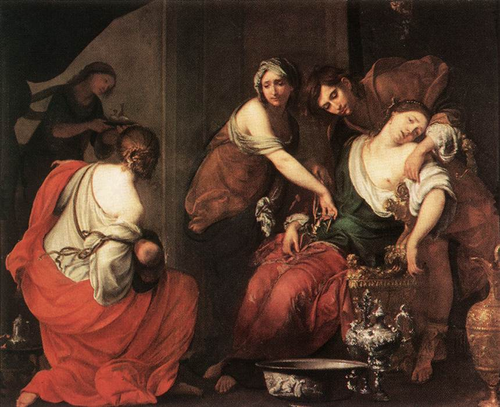
\includegraphics{./paintings_files/figure-pdf/cell-2-output-2.png}

Wikidata link: \url{http://www.wikidata.org/entity/Q29474644}

Title: Venetian Gala Concert

Year: 1782

Creator: Francesco Guardi

Copyright: public domain

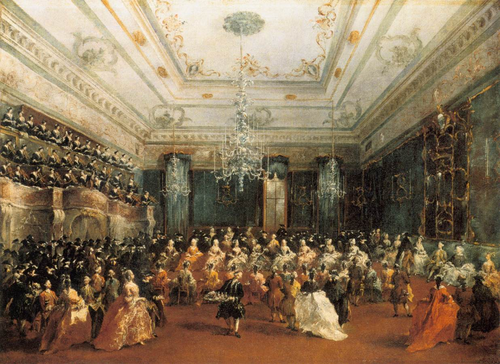
\includegraphics{./paintings_files/figure-pdf/cell-2-output-4.png}

Wikidata link: \url{http://www.wikidata.org/entity/Q29474645}

Title: Q29474645

Year: 1789

Creator: Francesco Guardi

Copyright: public domain

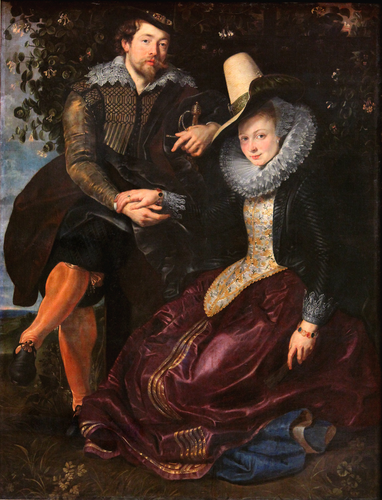
\includegraphics{./paintings_files/figure-pdf/cell-2-output-6.png}

\bookmarksetup{startatroot}

\hypertarget{introduction}{%
\chapter{Introduction}\label{introduction}}

This is a book created from markdown and executable code.

See Knuth (1984) for additional discussion of literate programming.

\bookmarksetup{startatroot}

\hypertarget{summary}{%
\chapter{Summary}\label{summary}}

In summary, this book has no content whatsoever.

\bookmarksetup{startatroot}

\hypertarget{references}{%
\chapter*{References}\label{references}}
\addcontentsline{toc}{chapter}{References}

\markboth{References}{References}

\hypertarget{refs}{}
\begin{CSLReferences}{1}{0}
\leavevmode\vadjust pre{\hypertarget{ref-knuth84}{}}%
Knuth, Donald E. 1984. {``Literate Programming.''} \emph{Comput. J.} 27
(2): 97--111. \url{https://doi.org/10.1093/comjnl/27.2.97}.

\end{CSLReferences}



\end{document}
